VTK has a long history of volume rendering and, unfortunately, that history is
evident in the large selection of classes available to render volumes. Each of
these methods was state-of-the-art at the time, but given VTK’s 20+ year
history, many of these methods are now quite obsolete. One of the goals of this
work is to reduce the number of volume mappers to ideally just two: one that
supports accelerated rendering on graphics hardware and another that works in
parallel on the CPU. The vtkSmartVolumeMapper would help application developers
by automatically choosing between these techniques based on system performance. 

\begin{figure}[h]
  \centering
  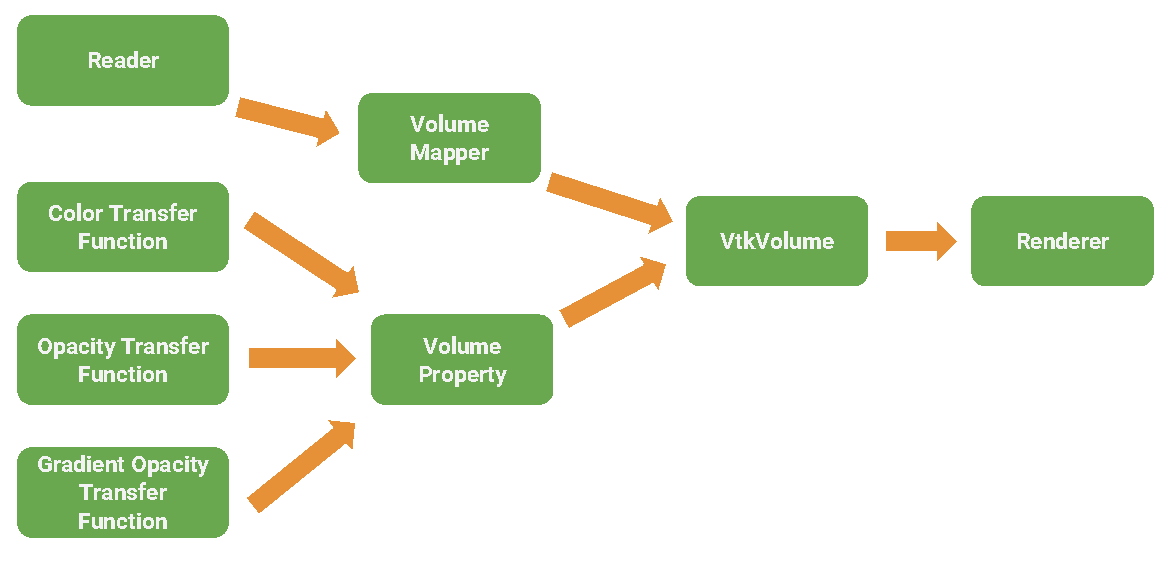
\includegraphics[width=\columnwidth]{vtk_volume_pipeline.pdf}
  \caption{VTK pipeline for volume rendering which is similar to VTK polygonal
    rendering with differences such as transfer functions are defined on the
    property object.}
  \label{fig:pipeline}
\end{figure}%

The main objective of this effort is to create a cross-platform,
multi-functional and high-performance volume renderer that works in both serial
and parallel mode (for example in
ParaView\cite{ahrens_paraview:_2005,ayachit_paraview_2015}). To achieve this,
we have created a replacement for the OpenGL fixed pipeline based
vtkGPUVolumeRayCastMapper. The new mapper, which shares the same name but uses
the OpenGL programmable pipeline, can be used via vtkSmartVolumeMapper or
instantiated directly and replaces the old vtkGPUVolumeRayCastMapper.
Availability of the new mapper with new OpenGL-VTK implementation improved the
management of textures in the mapper and benefited both forms of rendering
(geometry and volume) by sharing common code between them. While volume
ray-casting itself is a well-known technique, developing a volume renderer that
works with variety of data formats and types, supports many essential features
for medical and scientific computing, works on the main commercial platforms
(such as Windows, Mac, and Linux) and performs well at interactive frame rates
with very large datasets is still a challenging task that requires an in-depth
knowledge of the data, graphics pipeline, the VTK framework and the user
requirements.  In the next section, we will cover technical details of our work
that resulted in a sophisticated volume renderer for the VTK community.
